\documentclass[12pt,a4paper,twoside,openright]{book}


\usepackage[utf8]{inputenc}
\usepackage[T1]{fontenc}
\usepackage[english]{babel}
\usepackage{lmodern}


\usepackage{geometry}
\geometry{
    a4paper,
    top=3cm,
    bottom=3cm,
    left=2.5cm,
    right=2.5cm,
    heightrounded,
    bindingoffset=5mm,
    includehead,
    includefoot
}


\usepackage{amsmath}
\usepackage{amssymb}
\usepackage{amsthm}
\usepackage{amsfonts}
\usepackage{bm}


\usepackage{graphicx}
\usepackage[dvipsnames]{xcolor}
\usepackage{tikz}
\usetikzlibrary{positioning, arrows.meta, shapes.geometric, calc}


\usepackage{booktabs}
\usepackage{longtable}
\usepackage{tabularx}
\usepackage{array}


\usepackage{algorithm}
\usepackage{algpseudocode}

\algnewcommand\Inputs{\item[\textbf{Input:}]}
\algnewcommand\Outputs{\item[\textbf{Output:}]}
\algnewcommand\Initialization{\item[\textbf{Initialization:}]}


\usepackage{enumitem}


\usepackage{fancyhdr}
\setlength{\headheight}{14.5pt}
\pagestyle{fancy}
\fancyhf{}
\fancyhead[L]{\leftmark}
\fancyfoot[C]{\thepage}


\usepackage{hyperref}
\hypersetup{
    colorlinks=true,
    linkcolor=black,
    filecolor=magenta,
    urlcolor=Blue,
    pdftitle={My Personal Journey to Become an AI/ML Engineer - Riccardo Balzani},
    pdfpagemode=FullScreen,
}
\usepackage[all]{hypcap}


\newtheorem{theorem}{Theorem}[chapter]
\newtheorem{definition}{Definition}[chapter]
\newtheorem{lemma}{Lemma}[chapter]
\newtheorem{proposition}{Proposition}[chapter]
\newtheorem{corollary}{Corollary}[chapter]
\usepackage[most]{tcolorbox}

\newtcolorbox{unibobox}[1]{
  colback=red!5!white,
  colframe=red!75!black,
  fonttitle=\bfseries,
  title=#1,
  arc=4pt,
  outer arc=1pt
}

\title{My Personal Journey to Become an AI/ML Engineer}
\author{Riccardo Balzani (I'm still a student btw)}
\date{From January 2026}

\begin{document}

\maketitle

\tableofcontents

\chapter{The Mathematical Bedrock: Linear Algebra}

\begin{quote}
    \textit{"Linear Algebra is the language of modern AI. Without it, neural networks are just black boxes; with it, they are elegant geometric transformations."}
\end{quote}

\section*{A Note on Sources and Methodology}
The insights presented in this chapter are a synthesis of formal academic training and independent research. The core theoretical framework is built upon the lecture notes from the \textbf{Linear Algebra} course held by \textbf{Professor Luca Moci}.

These foundations were laid during my studies in \textbf{Computer Science and Engineering} at the \textbf{University of Bologna (Cesena Campus)}.

To bridge the gap between pure mathematical theory and practical AI applications, these academic roots have been integrated with:
\begin{itemize}
    \item \textbf{Textbook Reference:} \textit{Mathematics for Machine Learning} by Marc Peter Deisenroth, A. Aldo Faisal, and Cheng Soon Ong.
    \item \textbf{Digital Supplements:} Curated technical documentation and specialized online resources.
    \item \textbf{AI Collaboration:} Theoretical clarifications and synthesis facilitated by Large Language Models (LLMs) to explore advanced mathematical intuition.
\end{itemize}

\section{Vectors and Vector Spaces: The Atoms of Data}

In the context of Machine Learning, vectors are far more than mere geometric arrows; they are the fundamental containers for information. Whether we are representing a pixel in an image, a word in a sentence, or a user's preferences in a recommendation system, we are dealing with elements of a \textbf{Vector Space}.

\subsection{Formal Definition and Intuition}
Following a rigorous approach, we define a vector space $V$ over a field $\mathbb{R}$ as a set of objects (vectors) equipped with two operations: vector addition and scalar multiplication.

For ML engineers, the most relevant space is the $n$-dimensional Euclidean space $\mathbb{R}^n$. A vector $\mathbf{x} \in \mathbb{R}^n$ is an ordered $n$-tuple of real numbers:
$$ \mathbf{x} = \begin{bmatrix} x_1 \\ x_2 \\ \vdots \\ x_n \end{bmatrix} $$

\subsection{The Machine Learning Perspective}
Why does this matter in the labs? Because every "feature" of our dataset corresponds to a dimension in this space. If we are predicting house prices based on \textit{area} and \textit{number of rooms}, each house is a vector in $\mathbb{R}^2$.

As emphasized in \textit{Deisenroth's} work, the power of Linear Algebra lies in our ability to manipulate these high-dimensional objects using the same rules we use for simple 2D geometry. When we train a model, we are essentially looking for the "best" transformation or orientation within these abstract spaces.

\section{The Formal Structure of Vector Spaces}

To treat data as geometric objects, we must first define the algebraic structure that governs them. A \textbf{Vector Space} (or linear space) over a field $\mathbb{F}$ (typically the real numbers $\mathbb{R}$) is a set $V$ equipped with two binary operations that satisfy eight specific axioms.

\subsection{Formal Definition}
Let $V$ be a set and $\mathbb{F}$ be a field. We define two operations:
\begin{enumerate}
    \item \textbf{Vector Addition}: $+: V \times V \to V$, taking two vectors $\mathbf{u}, \mathbf{v}$ to a sum $\mathbf{u} + \mathbf{v}$.
    \item \textbf{Scalar Multiplication}: $\cdot: \mathbb{F} \times V \to V$, taking a scalar $a \in \mathbb{F}$ and a vector $\mathbf{v}$ to a product $a\mathbf{v}$.
\end{enumerate}

For $(V, \mathbb{F}, +, \cdot)$ to be a vector space, the following axioms must hold for all $\mathbf{u}, \mathbf{v}, \mathbf{w} \in V$ and all $a, b \in \mathbb{F}$:

\subsubsection*{Group Properties of Addition}
\begin{itemize}
    \item \textbf{Associativity}: $\mathbf{u} + (\mathbf{v} + \mathbf{w}) = (\mathbf{u} + \mathbf{v}) + \mathbf{w}$.
    \item \textbf{Commutativity}: $\mathbf{u} + \mathbf{v} = \mathbf{v} + \mathbf{u}$.
    \item \textbf{Identity element}: There exists an element $\mathbf{0} \in V$ such that $\mathbf{v} + \mathbf{0} = \mathbf{v}$.
    \item \textbf{Inverse element}: For every $\mathbf{v} \in V$, there exists $-\mathbf{v} \in V$ such that $\mathbf{v} + (-\mathbf{v}) = \mathbf{0}$.
\end{itemize}

\subsubsection*{Distributivity and Compatibility of Scalar Multiplication}
\begin{itemize}
    \item \textbf{Compatibility}: $a(b\mathbf{v}) = (ab)\mathbf{v}$.
    \item \textbf{Identity element}: $1\mathbf{v} = \mathbf{v}$, where $1$ is the multiplicative identity in $\mathbb{F}$.
    \item \textbf{Distributivity over vector addition}: $a(\mathbf{u} + \mathbf{v}) = a\mathbf{u} + a\mathbf{v}$.
    \item \textbf{Distributivity over field addition}: $(a + b)\mathbf{v} = a\mathbf{v} + b\mathbf{v}$.
\end{itemize}

\subsection{Significance in Engineering and Machine Learning}

The abstract nature of these axioms is not a mathematical pedantry but a functional necessity. By abstracting the concept of a "vector," we gain a unified framework to manipulate diverse data structures—be it a grayscale image ($I \in \mathbb{R}^{m \times n}$), a sequence of audio samples, or the hidden states of a Transformer model.

In Machine Learning, this provides the mathematical justification for two fundamental operations:

\begin{enumerate}
    \item \textbf{Feature Engineering and Interpolation}: If our data points reside in a vector space, we can compute their linear combinations. This allows us to perform "vector arithmetic" on concepts (e.g., in Word Embeddings, where $\vec{king} - \vec{man} + \vec{woman} \approx \vec{queen}$).
    \item \textbf{Parameter Optimization}: Training an AI model involves navigating a high-dimensional loss landscape. Because the parameters $\theta$ are vectors in a linear space, we can use Gradient Descent to "move" in a specific direction, confident that any step we take results in a valid set of parameters within that same space.
\end{enumerate}



\begin{unibobox}{The Closure Property}
    The most critical takeaway for an engineer is the \textbf{Closure Property}. It guarantees that for any $\mathbf{u}, \mathbf{v} \in V$, then $a\mathbf{u} + b\mathbf{v}$ is also in $V$. Without this, operations like the \textit{Stochastic Gradient Descent} update rule or calculating a weighted average of model weights (as seen in Federated Learning or Model Merging) would be mathematically undefined.
\end{unibobox}


\section{Linear Independence, Span, and Basis}

If vectors are the atoms of our data, then \textbf{Linear Combinations} are the molecules. Understanding how vectors interact to fill a space is fundamental for dimensionality reduction and understanding model capacity.

\subsection{Linear Combinations and Span}
A vector $\mathbf{v}$ is a \textbf{linear combination} of a set of vectors $\{\mathbf{v}_1, \dots, \mathbf{v}_k\}$ if there exist scalars $c_1, \dots, c_k \in \mathbb{F}$ such that:
\begin{equation}
    \mathbf{v} = c_1\mathbf{v}_1 + c_2\mathbf{v}_2 + \dots + c_k\mathbf{v}_k = \sum_{i=1}^k c_i\mathbf{v}_i
\end{equation}

The set of all possible linear combinations of $\{\mathbf{v}_1, \dots, \mathbf{v}_k\}$ is called the \textbf{Span}. In Machine Learning, the span of our features defines the "representational power" of a linear model; the model can only predict values that lie within the span of its input features.



\subsection{Linear Independence}
A set of vectors $\{\mathbf{v}_1, \dots, \mathbf{v}_k\}$ is \textbf{linearly independent} if the only way to satisfy the equation:
\begin{equation}
    \sum_{i=1}^k c_i\mathbf{v}_i = \mathbf{0}
\end{equation}
is by setting all coefficients to zero ($c_1 = c_2 = \dots = c_k = 0$).

If any vector in the set can be written as a linear combination of the others, the set is \textbf{linearly dependent}. From an engineering standpoint, dependence implies \textbf{redundancy}. In a dataset, if one feature is a linear combination of others (e.g., age in months vs. age in years), it adds no new information to the system and can lead to numerical instability during training.



\subsection{The Concept of a Basis}
A set of vectors $\mathcal{B} = \{\mathbf{b}_1, \dots, \mathbf{b}_n\}$ forms a \textbf{basis} for a vector space $V$ if:
\begin{enumerate}
    \item $\mathcal{B}$ is linearly independent.
    \item The span of $\mathcal{B}$ is equal to $V$ ($\text{span}(\mathcal{B}) = V$).
\end{enumerate}

The number of vectors in a basis is called the \textbf{Dimension} of the space. While we often use the standard basis (the identity axes), in AI we frequently search for *better* bases—such as the principal components in PCA—that align more effectively with the variance of our data.

\begin{unibobox}{Engineering Takeaway: The Curse of Redundancy}
    Linear dependence in your feature matrix $X$ leads to a \textbf{rank-deficient} matrix. This makes the matrix $X^TX$ non-invertible, causing the analytical solution for Linear Regression (the Normal Equation) to fail. Identifying linear independence is the first step in ensuring a model is "well-posed."
\end{unibobox}

\section{Linear Mappings and Matrices}

If vector spaces define the "stage," \textbf{Linear Mappings} are the movements that occur upon it. In AI, we rarely care about a static vector; we care about how that vector changes as it passes through the layers of a model.

\subsection{Defining the Linear Map}
A mapping $L: V \to W$ between two vector spaces is called \textbf{linear} if it preserves the structure of the space. Specifically, for all $\mathbf{u}, \mathbf{v} \in V$ and $c \in \mathbb{F}$, it must satisfy:
\begin{enumerate}
    \item \textbf{Additivity}: $L(\mathbf{u} + \mathbf{v}) = L(\mathbf{u}) + L(\mathbf{v})$
    \item \textbf{Homogeneity}: $L(c\mathbf{v}) = cL(\mathbf{v})$
\end{enumerate}



In simpler terms, a linear map ensures that the origin remains fixed and that straight lines remain straight and parallel after the transformation.
\begin{figure}[H]
    \centering
    
\includegraphics[width=0.7\linewidth]{img_cap1/Linear_Map.png}
    \caption{Kernel and image of a linear mapping $\Phi : V \rightarrow W$}
    \label{fig:placeholder}
\end{figure}

\subsection{Matrices as Operators}
While a linear map is an abstract concept, a \textbf{Matrix} is its concrete representation. Given a basis, every linear mapping $L: \mathbb{R}^n \to \mathbb{R}^m$ can be written as a matrix $A \in \mathbb{R}^{m \times n}$. The transformation of a vector $\mathbf{x}$ is computed via matrix-vector multiplication:
\begin{equation}
    \mathbf{y} = A\mathbf{x}
\end{equation}

A fundamental intuition in ML is viewing $A\mathbf{x}$ as a \textbf{linear combination of the columns of $A$}, weighted by the components of $\mathbf{x}$:
\begin{equation}
    A\mathbf{x} = x_1 \mathbf{a}_1 + x_2 \mathbf{a}_2 + \dots + x_n \mathbf{a}_n
\end{equation}



\subsection{Composition and Matrix Multiplication}
When we stack layers in a neural network, we are performing a \textbf{composition} of linear mappings. If $L$ is followed by $M$, the resulting transformation is represented by the product of their matrices $C = BA$. It is vital to remember that matrix multiplication is \textbf{non-commutative} ($AB \neq BA$); the \textbf{order of operations} in our data pipeline \textbf{matters}.

\begin{unibobox}{The "Hidden" Reality of AI Layers}
    In a standard Fully Connected layer, we compute $\mathbf{h} = \sigma(W\mathbf{x} + \mathbf{b})$. The term $W\mathbf{x}$ is a linear mapping that rotates and scales the input data into a new space (the hidden representation). The "learning" process is simply the systematic adjustment of the entries in matrix $W$ to find the transformation that best aligns the input with the desired output.
\end{unibobox}

\paragraph{Matrix and Vector Multiplication: The Inner Dimension Rule}

Matrix multiplication is not performed element-wise, but rather through a row-by-column dot product. For the product $AB$ of two matrices to be defined, the number of columns in the first matrix must match the number of rows in the second matrix. This is often referred to as the \textbf{inner dimension rule}: if matrix $A$ has dimensions $(n \times m)$ and matrix $B$ has dimensions $(m \times p)$, the "inner" dimensions ($m$) must be identical. The resulting matrix $C$ will then take the "outer" dimensions, resulting in an $(n \times p)$ matrix.



This principle extends naturally to \textbf{vector-matrix multiplication} by treating vectors as matrices with one dimension equal to 1. For a row vector $v$ to multiply a matrix $M$ from the left, its dimensions must be $(1 \times m)$ to match an $(m \times p)$ matrix. Conversely, for a matrix to be multiplied by a column vector from the right, the matrix must be $(n \times m)$ and the vector $(m \times 1)$. If these central dimensions do not align, the operation is mathematically undefined.



\begin{itemize}
    \item \textbf{Matrix $\times$ Matrix:} $(n \times \mathbf{m}) \times (\mathbf{m} \times p) \to (n \times p)$
    \begin{figure}[H]
        \centering
        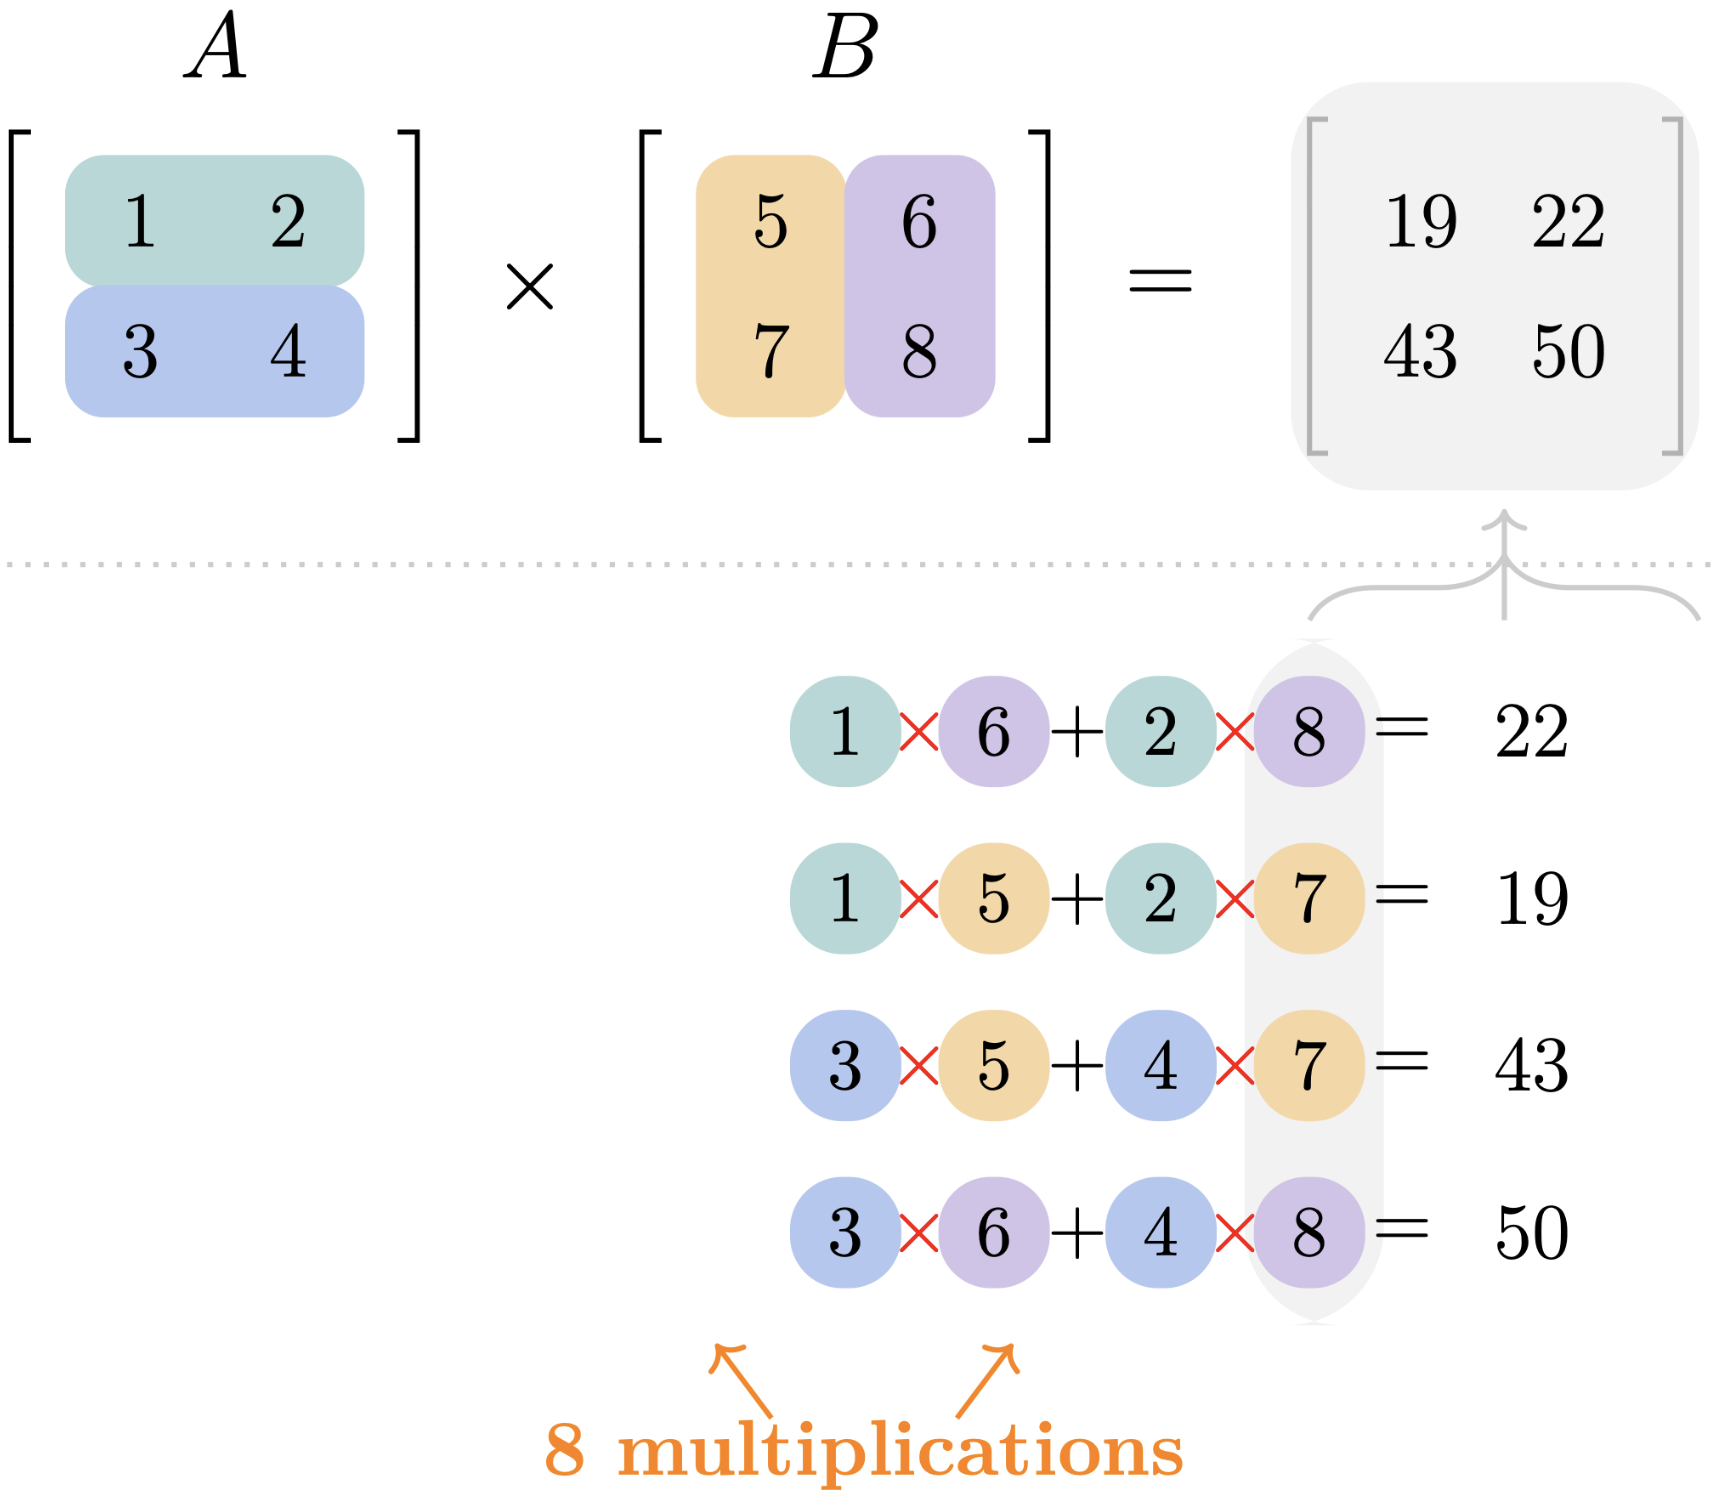
\includegraphics[width=0.5\linewidth]{img_cap1/matrix_mult.png}
        \caption{Example of $M_1 \times M_2$}
        \label{fig:placeholder}
    \end{figure}

    \item \textbf{Matrix $\times$ Column Vector:} $(n \times \mathbf{m}) \times (\mathbf{m} \times 1) \to (n \times 1)$
    \begin{figure}[H]
        \centering
        
\includegraphics[width=0.6\linewidth]{img_cap1/matric_vector.png}
        \caption{Example of $M \times v$}
        \label{fig:placeholder}
    \end{figure}
    \item \textbf{Row Vector $\times$ Matrix:} $(1 \times \mathbf{m}) \times (\mathbf{m} \times p) \to (1 \times p)$
    \begin{figure}[H]
        \centering
        
\includegraphics[width=0.8\linewidth]{img_cap1/row_vec_mat.png}
        \caption{Example of $v^T \times M$}
        \label{fig:placeholder}
    \end{figure}

    \item \textbf{Row Vector $\times$ Column Vector:} $(n \times \mathbf{1}) \times (\mathbf{1} \times p) \to (n \times p)$
    \begin{figure}[H]
        \centering
        
\includegraphics[width=0.8\linewidth]{img_cap1/row_column.png}
        \caption{Example of $u^T\times v$}
        \label{fig:placeholder}
    \end{figure}
\end{itemize}

\subsection{Matrices as Geometric Operators}

Until now, we have treated matrices and vectors primarily as data containers and tools for algebraic calculation (the classic "row-by-column" approach). However, for an AI Engineer, this view is limiting.

To truly understand what happens inside a neural network, we must shift our perspective: we should not view a matrix as a static table of numbers, but as a \textbf{dynamic function} that acts upon space.

When we compute the product $y = Ax$, matrix $A$ is "taking" vector $x$ and moving it to a new position. More formally, a matrix acts as an operator that transforms the grid of the vector space. This transformation can be decomposed into three fundamental actions:

\begin{enumerate}
    \item \textbf{Rotation:} The vector is rotated around the origin without changing its length.
    \item \textbf{Scaling (Dilation/Contraction):} The vector is stretched or shrunk along the axes.
    \item \textbf{Shear:} The space is "slanted," transforming squares into rhombuses.
\end{enumerate}

The key intuition is this: \textbf{the columns of matrix $A$ tell us exactly where the standard basis vectors land after the transformation.}

If we have a matrix $A = \begin{bmatrix} 2 & -1 \\ 0 & 1 \end{bmatrix}$:
\begin{itemize}
    \item The first column $\begin{bmatrix} 2 \\ 0 \end{bmatrix}$ tells us that the basis vector $\hat{i}$ (which was at $[1, 0]$) is stretched to the coordinates $[2, 0]$.
    \item The second column $\begin{bmatrix} -1 \\ 1 \end{bmatrix}$ tells us that the basis vector $\hat{j}$ (which was at $[0, 1]$) is moved to $[-1, 1]$.
\end{itemize}

The entire space is deformed accordingly.

\begin{unibobox}{Engineering Insight: Deep Learning as Data "Origami"}
This geometric interpretation is the secret to understanding Deep Neural Networks.

Imagine a classification dataset (e.g., images of cats and dogs) distributed in space. Often, these data are "tangled" in complex ways and are not separable by a simple straight line (they are not linearly separable).

Every layer of a neural network (Fully Connected) applies a transformation $Wx + b$.
\begin{itemize}
    \item The weight matrix $W$ applies a linear transformation (rotating, scaling, and stretching the space).
    \item The activation function (e.g., ReLU) applies a non-linear "fold."
\end{itemize}

We can view the training of a neural network as the attempt to find that specific sequence of matrices that "stretches," "rotates," and "deforms" the data space until points of different classes (cats and dogs) are untangled and pushed into different regions of the space, where they finally become easy to separate.
\end{unibobox}

\subsection{Rank and Data Compression}

The concept of \textbf{Rank} connects linear algebra directly to information theory.
While the dimensions of a matrix tell us how much memory it occupies (e.g., a $1000 \times 1000$ matrix has 1 million entries), the \textbf{Rank} tells us how much \textit{information} it actually carries.

\paragraph{Formal Definition:} The rank of a matrix is the maximum number of linearly independent columns (or rows).
\paragraph{Geometric Interpretation:} It is the dimension of the output space after the transformation. If a $3 \times 3$ matrix has Rank 2, it collapses the entire 3D space onto a flat 2D plane. If it has Rank 1, it collapses everything onto a single line.

\paragraph{The Concept of "Low-Rank":}
In Machine Learning, we often deal with high-dimensional data that is highly redundant. A large matrix is said to be "Low-Rank" if it can be factorized into much smaller matrices without losing significant information. This implies that even though the data lives in a high-dimensional space, its underlying structure is simple.

\begin{unibobox}{Engineering Insight: LoRA (Low-Rank Adaptation)}
The most impactful application of rank in modern AI is \textbf{LoRA}, a technique used to fine-tune Large Language Models (LLMs).

When we want to teach a pre-trained model a new task, we theoretically need to update its weight matrix $W$ (which might have billions of parameters). However, researchers found that the update matrix $\Delta W$ has a very \textbf{low intrinsic rank}.

Instead of retraining the massive matrix $W$, LoRA trains two tiny matrices $A$ and $B$ such that the update is approximated by their product: $\Delta W \approx A \times B$.
For a $4096 \times 4096$ weight matrix (over 16 million parameters), a Rank-8 LoRA adapter only needs to learn roughly $65,000$ parameters. This allows engineers to fine-tune huge models on consumer hardware.
\end{unibobox}

\subsubsection*{Example: Calculating Rank via Row Reduction}

To find the rank of a matrix manually, we perform Gaussian Elimination to reach the \textit{Row Echelon Form}. The rank is simply the count of non-zero rows remaining.

Consider the matrix $A$:

\begin{equation*}
A =
\begin{bmatrix}
1 & 2 & 3 \\
2 & 4 & 6 \\
0 & 1 & 5
\end{bmatrix}
\end{equation*}

\textbf{Step 1: Identify Redundancy.}
Notice that the second row is exactly twice the first row ($R_2 = 2 \times R_1$). This implies linear dependence. We apply the operation $R_2 \leftarrow R_2 - 2R_1$:

\begin{equation*}
\xrightarrow{R_2 - 2R_1}
\begin{bmatrix}
1 & 2 & 3 \\
\mathbf{0} & \mathbf{0} & \mathbf{0} \\
0 & 1 & 5
\end{bmatrix}
\end{equation*}

\textbf{Step 2: Reorder to Echelon Form.}
We swap the zero row with the non-zero row below it ($R_2 \leftrightarrow R_3$) to organize the matrix:

\begin{equation*}
\xrightarrow{swap}
\begin{bmatrix}
1 & 2 & 3 \\
0 & 1 & 5 \\
\mathbf{0} & \mathbf{0} & \mathbf{0}
\end{bmatrix}
\end{equation*}

\textbf{Conclusion:}
We have \textbf{2} non-zero rows remaining (the pivots are highlighted).
\[
\text{Rank}(A) = 2
\]
This tells us that the input space was 3-dimensional, but the matrix collapses it onto a 2-dimensional plane.

\subsection{The Determinant as a Volume Measure}

The determinant of a square matrix $A$, denoted as $det(A)$ or $|A|$, is often introduced as a complex recursive calculation (Laplace expansion) \footnote{\textbf{Laplace Expansion:} A recursive method to compute the determinant. By expanding along any fixed row $i$, the formula is:
$ \det(A) = \sum_{j=1}^{n} (-1)^{i+j} a_{ij} M_{ij} $
where $a_{ij}$ is the element at row $i$ and column $j$, and $M_{ij}$ (the \textit{Minor}) is the determinant of the $(n-1) \times (n-1)$ submatrix obtained by deleting row $i$ and column $j$.}. While knowing how to compute it is useful, understanding its geometric meaning is essential for AI.

\paragraph{Geometric Intuition:}
The determinant measures how much the linear transformation $A$ \textbf{scales the volume} of the space.
\begin{itemize}
    \item If $det(A) = 2$, the transformation doubles the area (in 2D) or volume (in 3D) of any shape.
    \item If $det(A) = 1$, the transformation preserves volume (like a pure rotation or shear).
    \item If $det(A) < 0$, the transformation involves flipping the orientation of space (like looking in a mirror).
\end{itemize}

\paragraph{The Case of Zero Determinant:}
The most critical value is $det(A) = 0$.
Geometrically, this means the transformation squashes the entire space into a lower dimension (e.g., flattening a 3D cube onto a 2D sheet). The volume becomes zero.
When this happens, information is lost forever, and the transformation is irreversible (the matrix is non-invertible or "singular").

\begin{unibobox}{Engineering Insight: Generative AI and Normalizing Flows}
In modern Generative AI, specifically in \textbf{Normalizing Flows}, we design complex neural networks that map a simple distribution (like a Gaussian) to a complex one (like images of faces).

To generate valid new data points, this mapping must be reversible (invertible). This leads to a strict design constraint: the Jacobian matrix of the layers must have a non-zero determinant.
Furthermore, to calculate the probability density of the generated images, we explicitly track the $\log(det(J))$. If the determinant collapses to zero, the model breaks because the probability density becomes undefined.
\end{unibobox}

\subsection{Inversion and Numerical Stability}

From a theoretical standpoint, the inverse of a square matrix $A$ is a powerful tool. It is the unique matrix $A^{-1}$ such that $A A^{-1} = I$. If we have a linear system $Ax = b$, the elegant analytical solution is simply $x = A^{-1}b$.

However, in the practical world of Engineering, computing the explicit inverse is often considered a "numerical crime."

There are two main reasons for this reluctance:
\begin{enumerate}
    \item \textbf{Computational Complexity:} Algorithms to invert a matrix typically scale with $O(n^3)$. As $n$ grows (e.g., in a neural network layer with thousands of neurons), the computation time becomes prohibitive.
    \item \textbf{Numerical Stability:} Computers use floating-point arithmetic, which has finite precision. The process of inversion tends to accumulate rounding errors, leading to results that can be wildly inaccurate.
\end{enumerate}

\begin{unibobox}{Engineering Insight: Don't Invert... Solve!}
In Python libraries like NumPy or PyTorch, you will often see two functions: \texttt{inv(A)} and \texttt{solve(A, b)}.

\textbf{Best Practice:} Always prefer \texttt{solve(A, b)}.
Instead of computing the full inverse matrix and then multiplying, \texttt{solve} uses optimized algorithms (like LU decomposition) to find $x$ directly. It is faster and more precise.

\textbf{The Condition Number:}
To quantify the stability of a matrix, we use the \textit{Condition Number}, denoted as $\kappa(A)$.
\[
\kappa(A) = ||A|| \cdot ||A^{-1}||
\]
It measures how much the output value $x$ changes for a small change in the input $b$ (noise).
\begin{itemize}
    \item If $\kappa(A)$ is low (close to 1), the matrix is \textbf{well-conditioned}.
    \item If $\kappa(A)$ is very high (e.g., $10^5$), the matrix is \textbf{ill-conditioned}. In this case, calculating the inverse will amplify the numerical noise, rendering the result useless.
\end{itemize}
\end{unibobox}

\section{Norms and Inner Products: The Geometry of Similarity}

While linear mappings define how we transform data, \textbf{Norms} and \textbf{Inner Products} allow us to quantify the "size" of vectors and the "closeness" between them. In Machine Learning, these tools are the backbone of loss functions and similarity metrics.

\subsection{Inner Products and Geometry}
An \textbf{Inner Product} is a function that takes two vectors and returns a scalar, providing a notion of angle and length. For $\mathbf{u}, \mathbf{v} \in \mathbb{R}^n$, the standard inner product (\textbf{dot product}) is defined as:
\begin{equation}
    \langle \mathbf{u}, \mathbf{v} \rangle = \mathbf{u}^\top \mathbf{v} = \sum_{i=1}^n u_i v_i
\end{equation}



The inner product is intrinsically linked to the angle $\theta$ between vectors:
\begin{equation}
    \langle \mathbf{u}, \mathbf{v} \rangle = \|\mathbf{u}\| \|\mathbf{v}\| \cos(\theta)
\end{equation}
In AI, this leads directly to \textbf{Cosine Similarity}, a standard metric for comparing word embeddings or document vectors, where the magnitude of the vectors is often less important than their direction.

\subsection{Case Study: Numerical Similarity in Feature Spaces}

Consider a simplified 2D feature space where the axes represent \textbf{Tech} and \textbf{Fruitness}. We can represent objects as vectors $\mathbf{x} = [x_{tech}, x_{fruit}]^\top$. For instance:
\begin{itemize}
    \item \textbf{Cherries}: $[1, 4]^\top$
    \item \textbf{Orange}: $[0, 3]^\top$
    \item \textbf{Smartphone}: $[3, 0]^\top$
\end{itemize}

\begin{figure}[H]
    \centering
    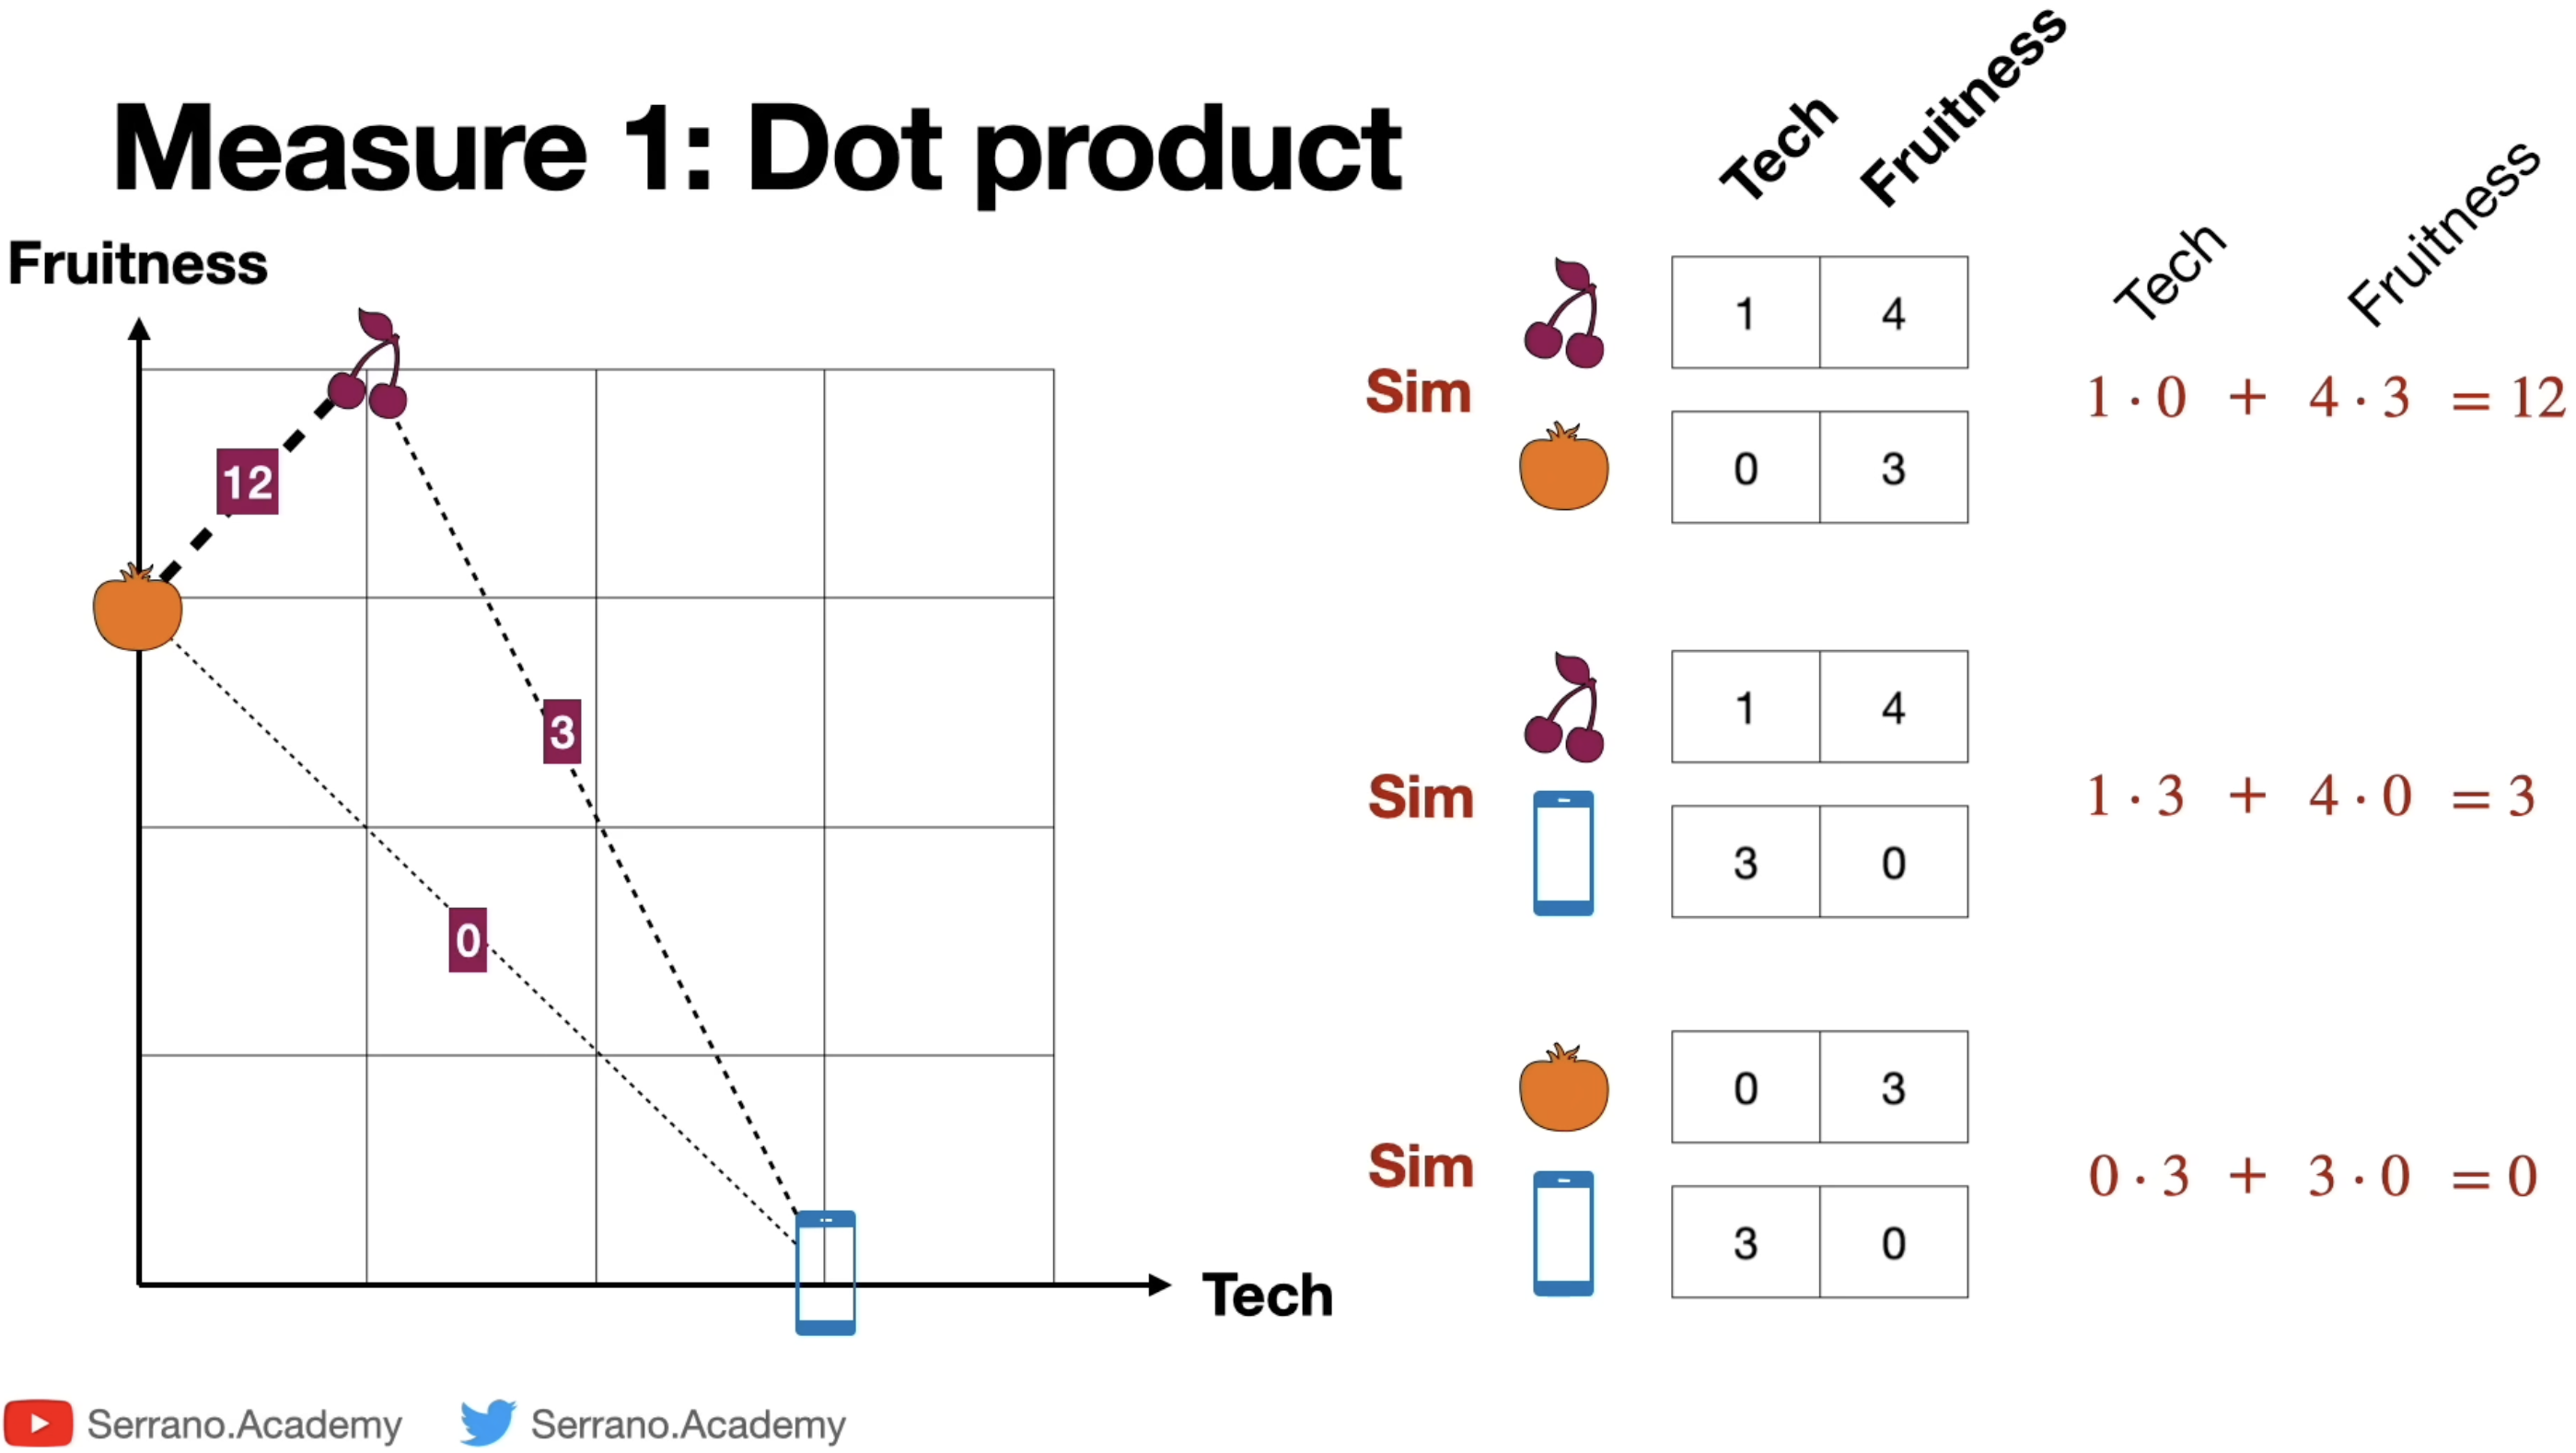
\includegraphics[width=0.9\textwidth]{img_cap1/Inner_prod_similarity.png}
    \caption{Numerical calculation of the Dot Product. By computing the sum of element-wise products, we see that "Cherries" and "Oranges" have the highest alignment (12), while "Oranges" and "Smartphones" have a dot product of 0, indicating they share no common features in this basis.}
    \label{fig:dot_calc}
\end{figure}

\begin{figure}[H]
    \centering
    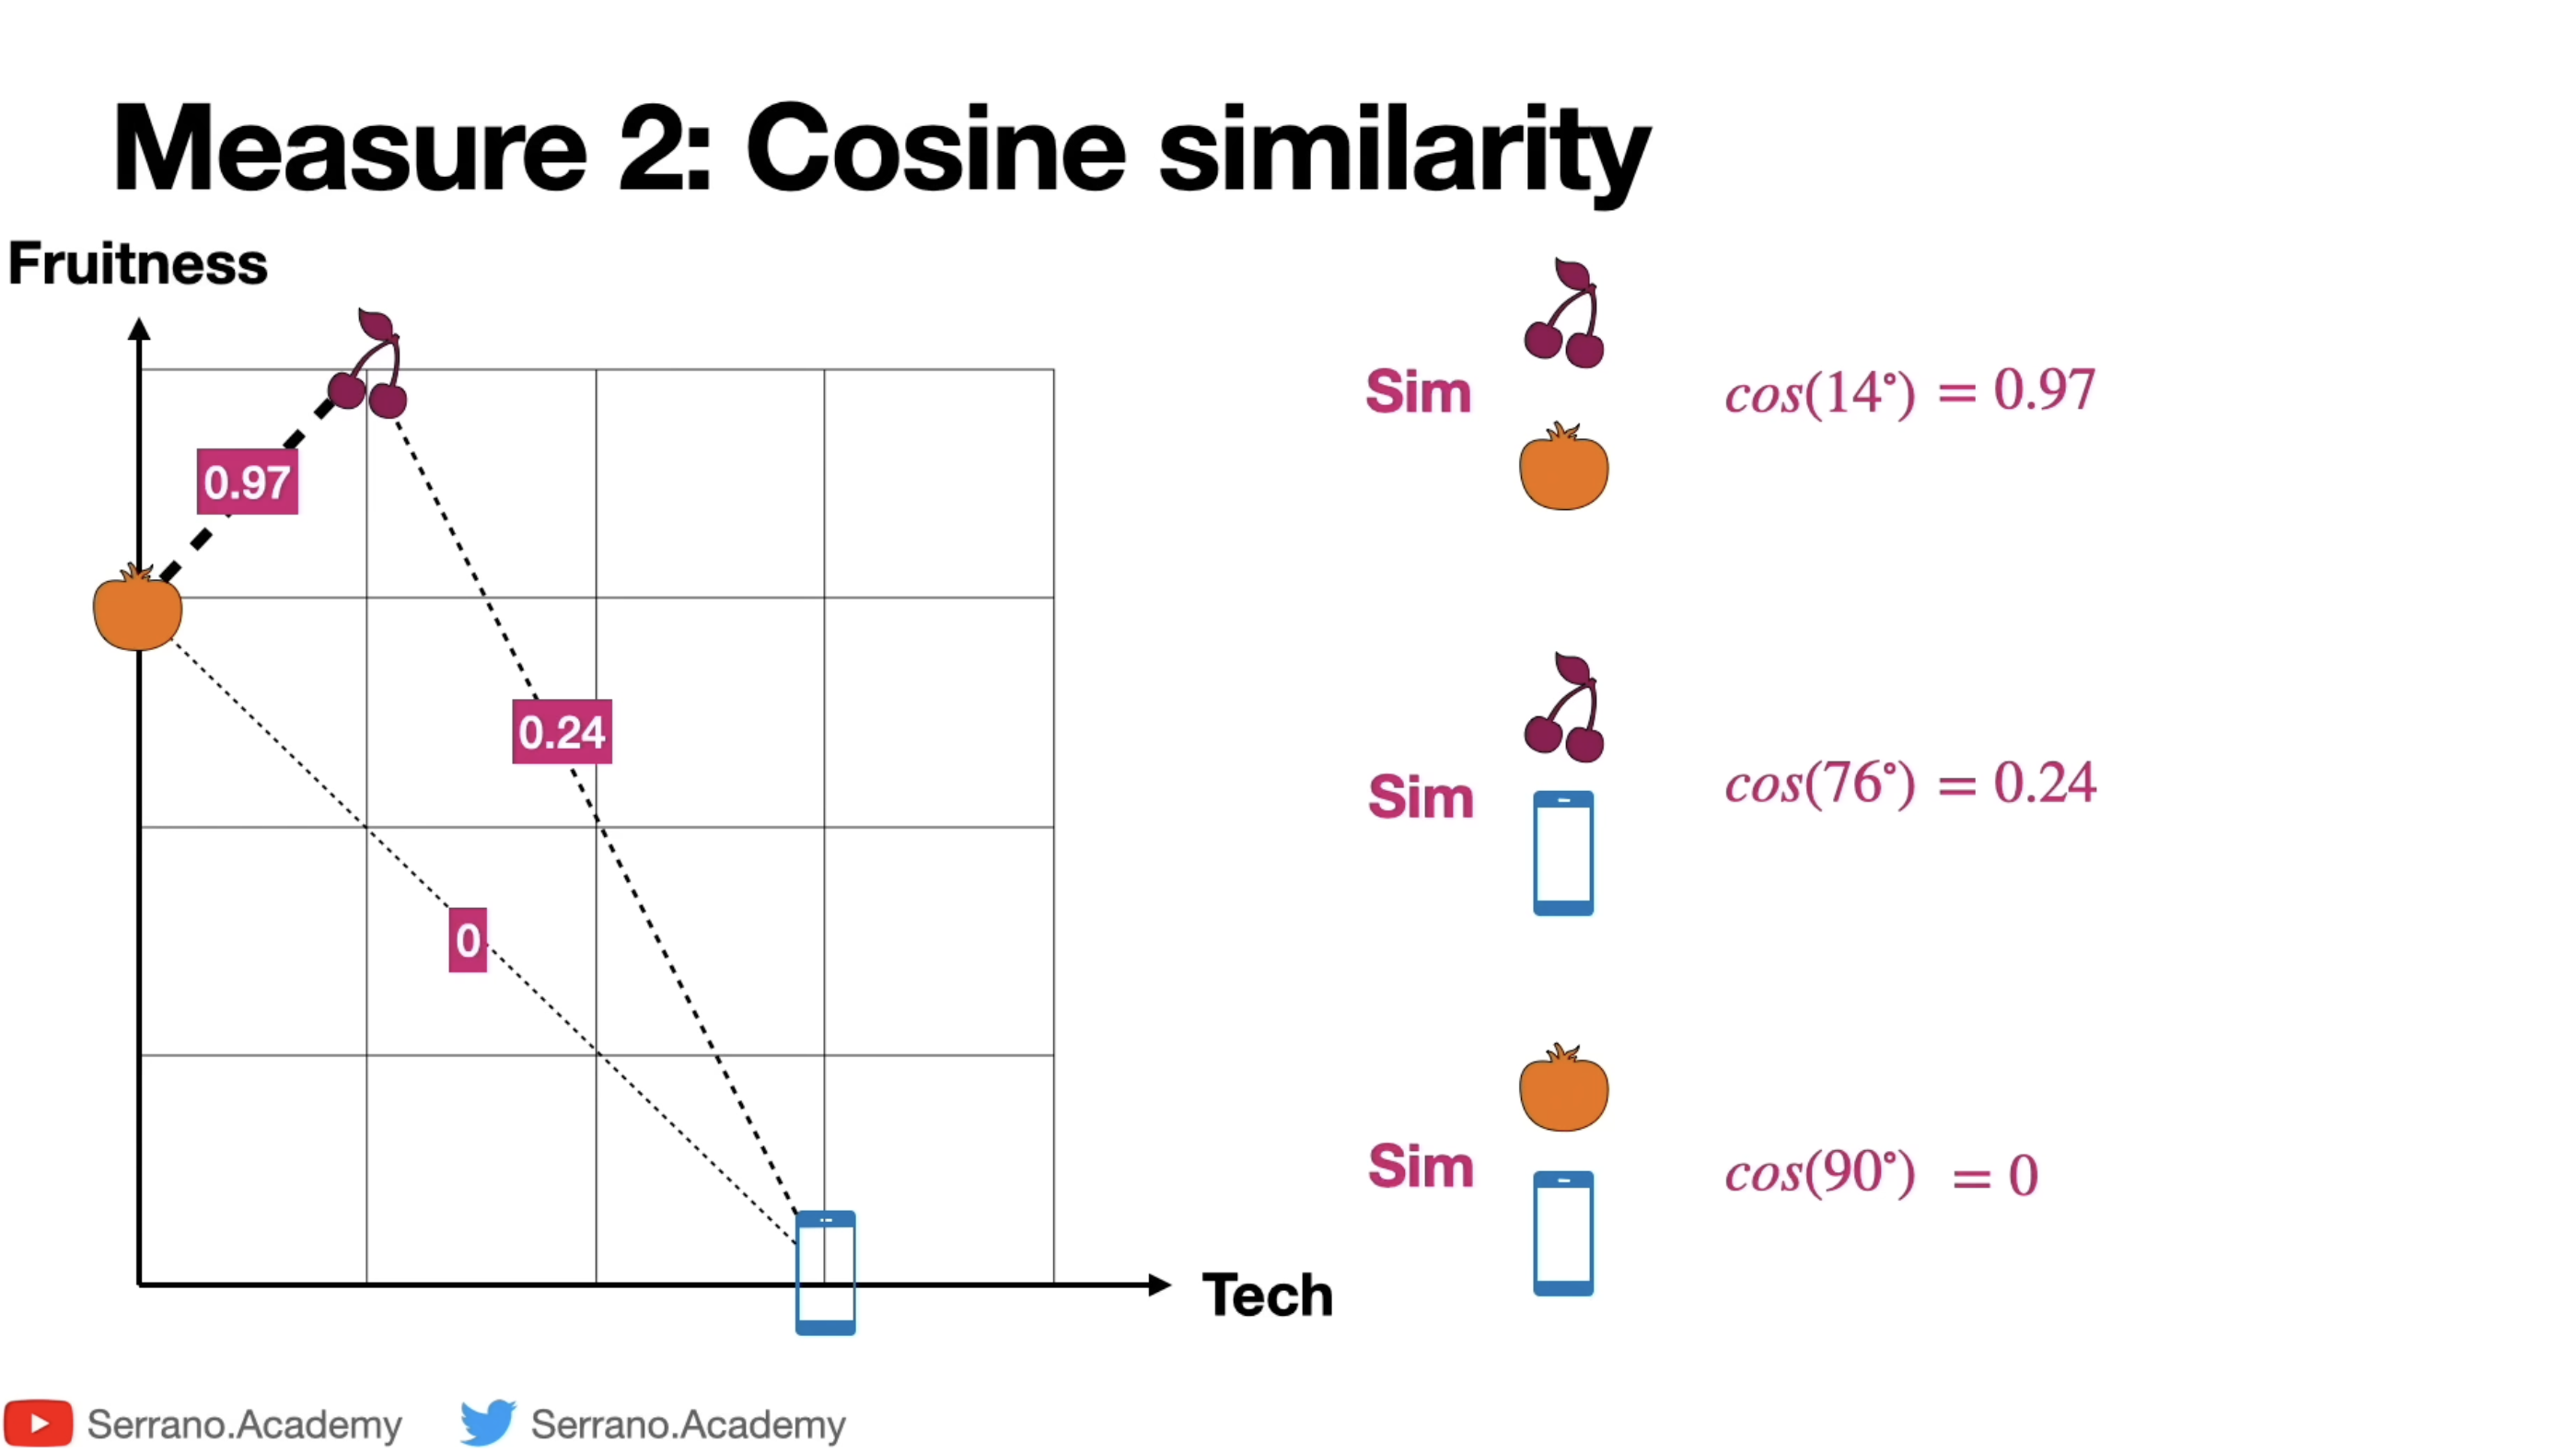
\includegraphics[width=0.9\textwidth]{img_cap1/cosine_similarity.png}
    \caption{Numerical calculation of Cosine Similarity. Notice how the raw dot product scores are normalized by the magnitudes of the vectors. This results in a similarity of $0.97$ for the two fruits, providing a magnitude-invariant measure of their relationship.}
    \label{fig:cosine_calc}
\end{figure}

\begin{unibobox}{Insight: Orthogonality as Independence}
    When the dot product between the "Orange" and "Smartphone" vectors is exactly $0$, we say they are \textbf{orthogonal}. In the context of data, this means the two variables are linearly independent; knowing how "fruity" an object is gives us zero information about how "technological" it is. This is the ideal state for features in a well-conditioned machine learning model.
\end{unibobox}

\subsection{The Bridge: Normalization and Equivalence}

A critical insight in data preprocessing is the relationship between the dot product and cosine similarity. As visualized in Figure \ref{fig:normalization_bridge}, these two metrics become identical when the vectors are \textbf{normalized} to unit length (i.e., $\|\mathbf{x}\| = 1$).

\begin{figure}[H]
    \centering
    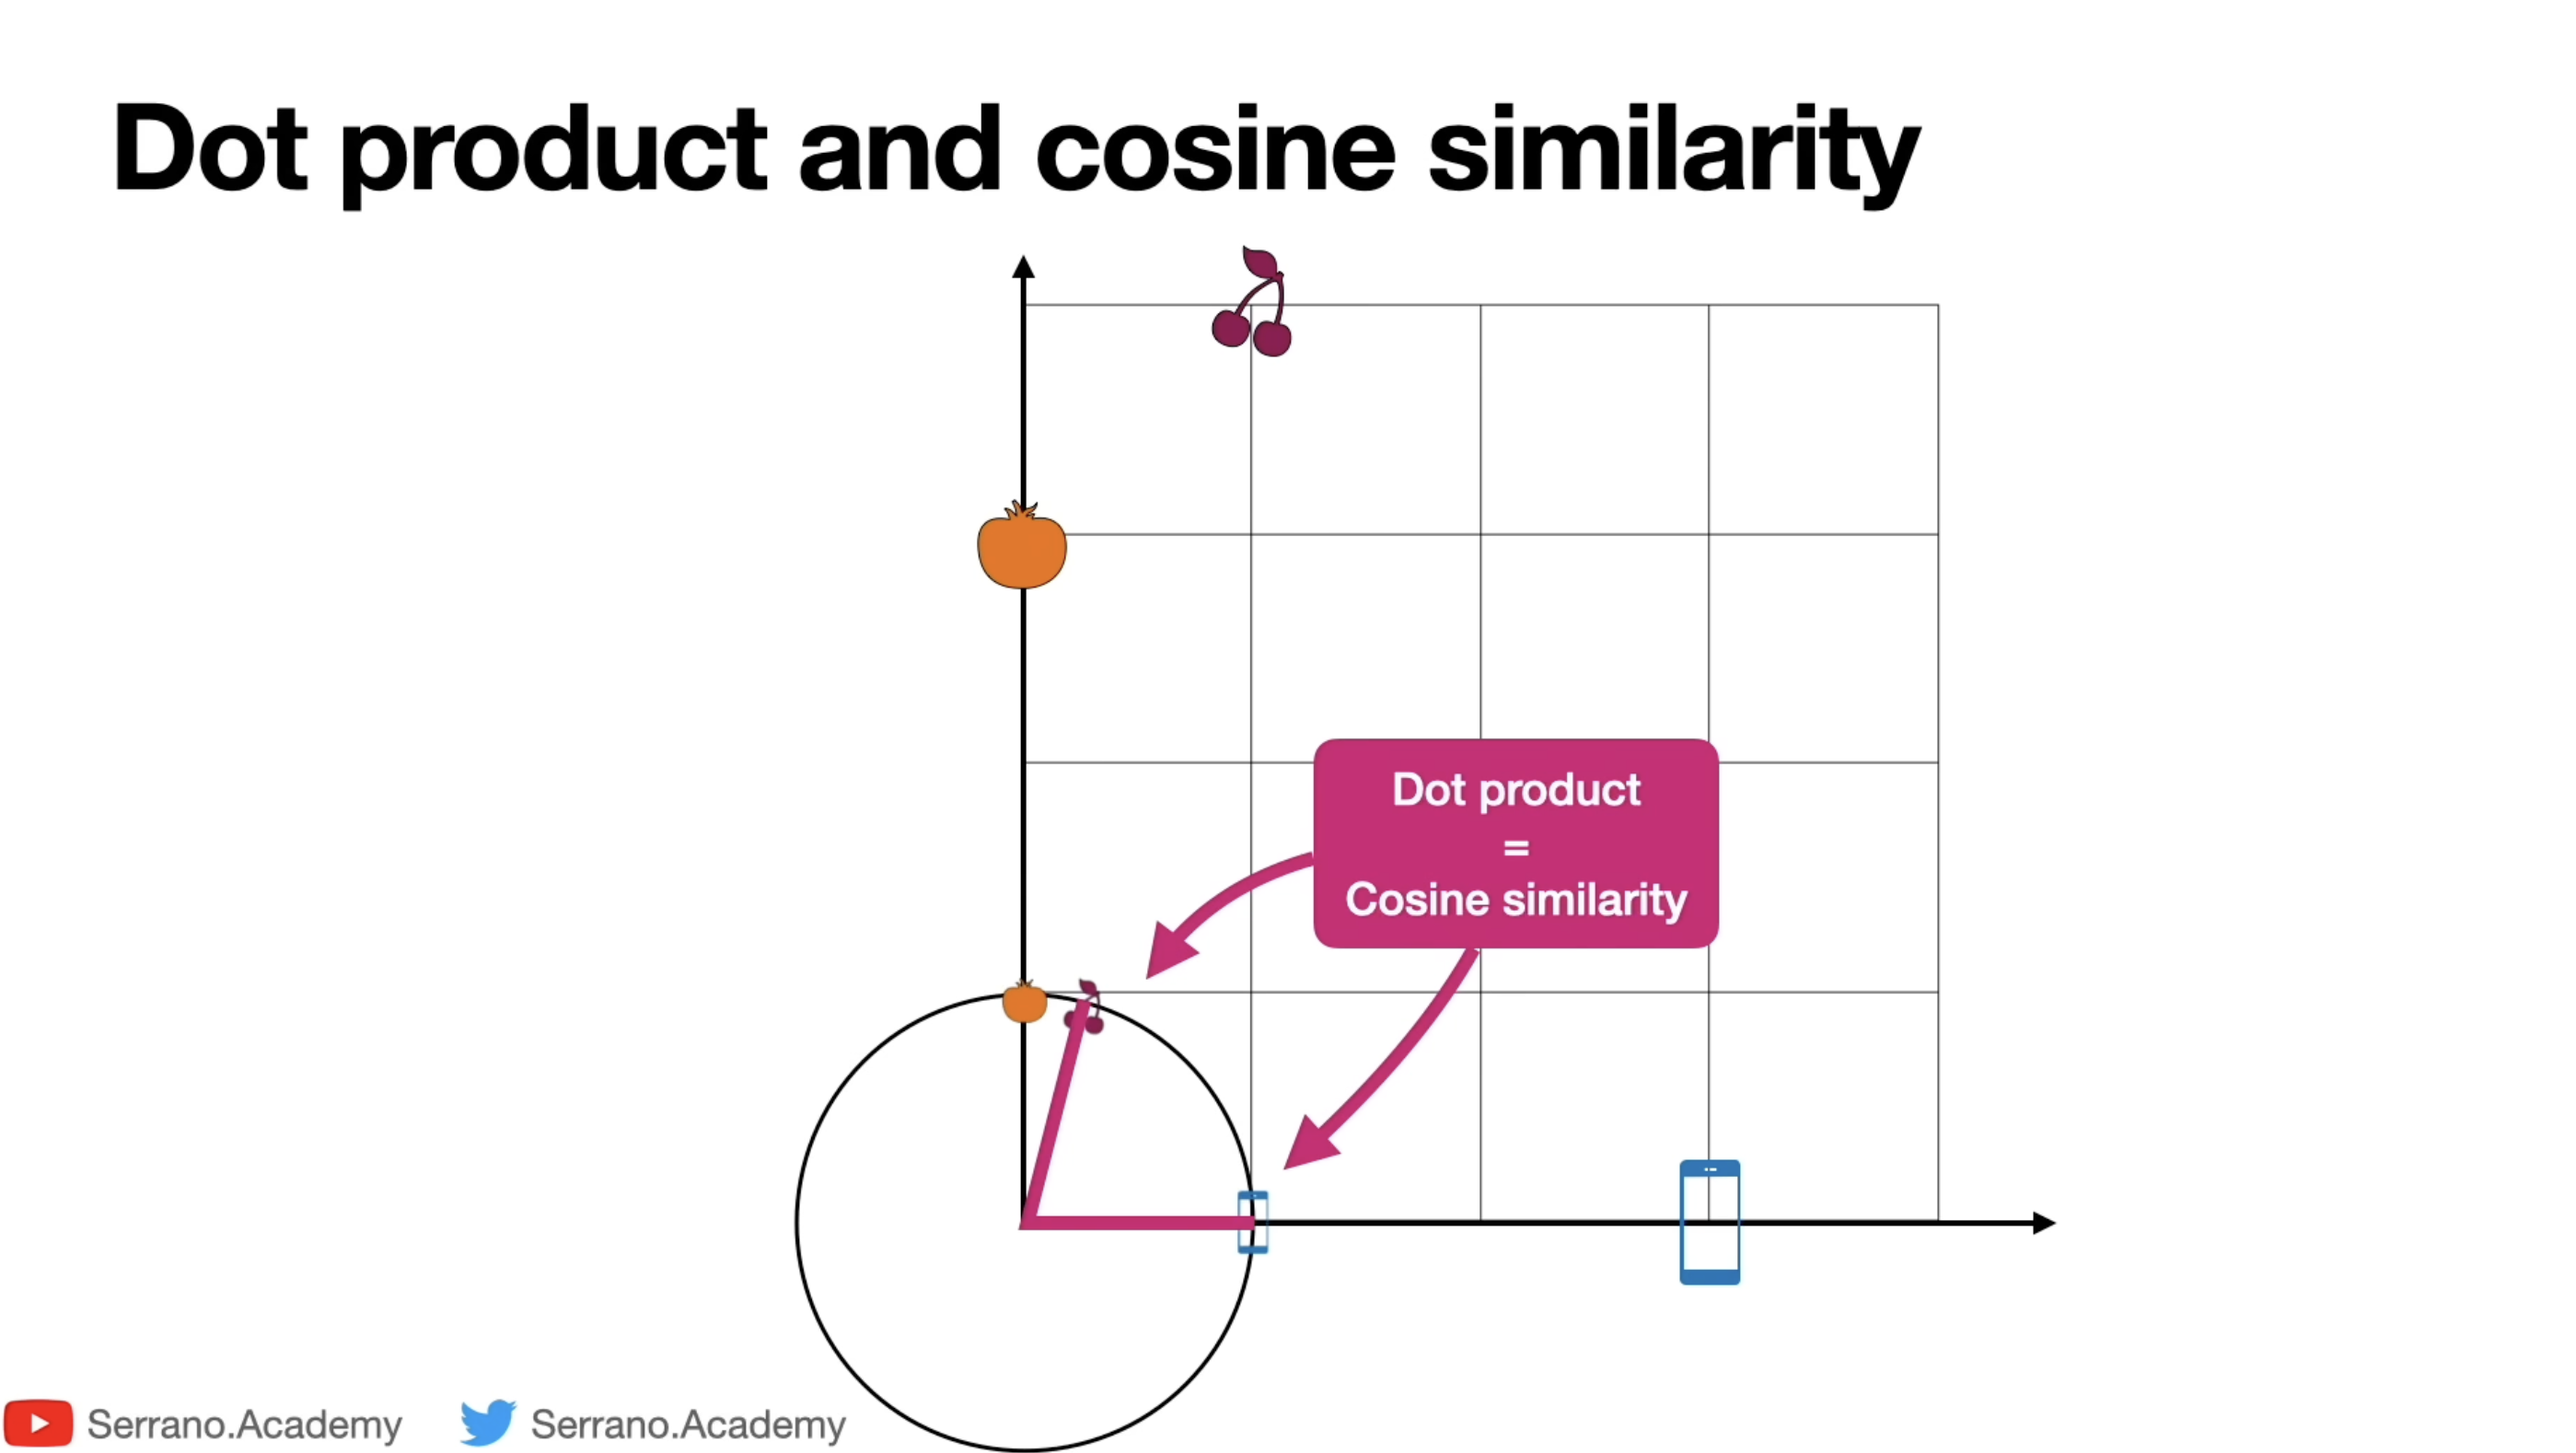
\includegraphics[width=0.8\textwidth]{img_cap1/cosine_inner.png}
    \caption{The relationship between Dot Product and Cosine Similarity. When vectors are projected onto a unit circle (normalized), their magnitude becomes 1, and the dot product calculation yields the same value as the cosine similarity.}
    \label{fig:normalization_bridge}
\end{figure}

Mathematically, if we define the normalized version of a vector $\mathbf{u}$ as $\hat{\mathbf{u}} = \frac{\mathbf{u}}{\|\mathbf{u}\|}$ \footnote{\textbf{Equivalence between Dot Product and Cosine Similarity:} This identity holds \textit{only} if the vectors are normalized (i.e., they have unit norm $||u||=||v||=1$). From the geometric definition of the dot product $\langle u, v \rangle = ||u|| \cdot ||v|| \cdot \cos(\theta)$, substituting the norms with 1 immediately yields $\langle u, v \rangle = 1 \cdot 1 \cdot \cos(\theta) = \cos(\theta)$. Practically, normalizing data transforms the dot product into a pure measure of angular alignment.}, then:
\begin{equation}
    \text{Cosine Similarity}(\mathbf{u}, \mathbf{v}) = \langle \hat{\mathbf{u}}, \hat{\mathbf{v}} \rangle = \hat{\mathbf{u}}^\top \hat{\mathbf{v}}
\end{equation}


\begin{unibobox}{Engineering Insight: Preprocessing Matters}
    In many ML pipelines, we explicitly normalize our data (e.g., using \texttt{StandardScaler} or \texttt{Normalizer} in Scikit-Learn). We do this because raw dot products can be dominated by a single feature with a very large scale, which can "confuse" the model. By mapping data to the unit hypersphere, we ensure that the model learns the \textbf{structural patterns} (angles) of the data rather than being distracted by the \textbf{intensity} (magnitude).
\end{unibobox}

\subsection{Vector Norms}
A \textbf{Norm} $\|\cdot\|$ is a function that assigns a \textbf{strictly positive length} to a vector. The general $L_p$ norm is defined as:
\begin{equation}
    \|\mathbf{x}\|_p = \left( \sum_{i=1}^n |x_i|^p \right)^{1/p}
\end{equation}

In Engineering, two specific norms dominate the landscape:
\begin{itemize}
    \item \textbf{$L_2$ Norm (Euclidean Norm)}: $\|\mathbf{x}\|_2 = \sqrt{\sum x_i^2}$. It represents the shortest distance between points.
    \item \textbf{$L_1$ Norm (Manhattan Norm)}: $\|\mathbf{x}\|_1 = \sum |x_i|$. It is the sum of absolute differences.
\end{itemize}



\subsection{Orthogonality}
Two vectors are \textbf{orthogonal} if their inner product is zero ($\langle \mathbf{u}, \mathbf{v} \rangle = 0$). In the context of features, orthogonality means zero redundancy; the information contained in $\mathbf{u}$ cannot be explained by $\mathbf{v}$.

\begin{unibobox}{Engineering Application: Regularization}
    We use norms to prevent models from overfitting through \textbf{Regularization}:
    \begin{itemize}
        \item \textbf{$L_2$ Regularization (Ridge)}: Adds a penalty proportional to the square of the weights. This forces weights to be small but non-zero, promoting stability.
        \item \textbf{$L_1$ Regularization (Lasso)}: Adds a penalty proportional to the absolute value of the weights. Due to the "diamond" shape of the $L_1$ unit ball, this often forces some weights to exactly zero, performing automatic \textbf{Feature Selection}.
    \end{itemize}
\end{unibobox}

\section{The Spectral Perspective: Eigenvalues and Eigenvectors}

Up to this point, we have seen that a matrix $A$ acts as a machine that rotates and distorts vectors. In general, if you take a random vector $x$ and apply $A$ to it, the resulting vector $Ax$ will point in a completely different direction.

However, for every square matrix, there exist special "privileged" vectors that defy this rule. These are the \textbf{Eigenvectors}.

\subsection{Defining the Invariant Directions}

Geometrically, an eigenvector $v$ is a non-zero vector that does not change its orientation when transformed by $A$. The matrix effectively acts as a simple scalar multiplier on these specific vectors.
\paragraph{Formal Definition:}
A vector $v \in \mathbb{R}^n$ ($v \neq 0$) is an eigenvector of a square matrix $A$ if there exists a scalar $\lambda$ (lambda) such that:

\begin{equation}
Av = \lambda v
\end{equation}

Where:
\begin{itemize}
    \item $v$ is the \textbf{Eigenvector} ("Eigen" is German for "own" or "characteristic"). It represents the \textit{direction} of the axis.
    \item $\lambda$ is the \textbf{Eigenvalue}. It represents the \textit{magnitude} of the stretch.
\end{itemize}
\paragraph{Physical Intuition:}
Imagine the rotation of a 3D globe. Almost every vector pointing from the center to the surface moves and changes direction as the globe spins.
However, there is one vector that remains perfectly stationary: the axis of rotation (the North-South pole line). This axis is the eigenvector of the rotation matrix, and since it doesn't stretch or shrink, its eigenvalue is $\lambda = 1$.

In Engineering, finding the eigenvectors is equivalent to finding the "natural axes" of a system—the directions where the action happens independently from the others.

\subsection{AI Case Study: PCA (Principal Component Analysis)}

The most elegant application of eigenvectors in Machine Learning is undoubtedly \textbf{Principal Component Analysis (PCA)}.

In many real-world datasets, we suffer from the "Curse of Dimensionality": we have too many features (e.g., thousands of pixels in an image), but the actual meaningful information resides in a much lower-dimensional subspace.
The goal of PCA is to find the "best" way to compress this data while losing as little information as possible.

\textbf{The Core Idea: Variance is Information}
PCA assumes that "information" equates to "variance." If a feature is constant across all samples (variance = 0), it tells us nothing. If it varies wildly, it holds information.

\textbf{The Eigen-Connection:}
To find the directions where the data varies the most, we compute the \textbf{Covariance Matrix} ($\Sigma$) of our dataset. This matrix summarizes how every feature correlates with every other feature.
\begin{enumerate}
    \item We calculate the \textbf{eigenvectors} of the Covariance Matrix.
    \item These eigenvectors point exactly along the axes of maximum data spread. These are the \textbf{Principal Components}.
    \item The corresponding \textbf{eigenvalues} tell us the \textit{amount} of variance captured by that component.
\end{enumerate}

\begin{unibobox}{Engineering Insight: Dimensionality Reduction}
This provides a powerful algorithmic recipe for compression:
1. Compute the eigenvalues of your data's covariance matrix.
2. Sort them from largest to smallest ($\lambda_1 > \lambda_2 > \dots > \lambda_n$).
3. Keep only the top $k$ eigenvectors (e.g., the top 3) and discard the rest.

If the sum of the top 3 eigenvalues accounts for 95\% of the total sum, you can reduce your dataset from 1000 dimensions down to 3, while preserving 95\% of the original information. You have successfully separated the "signal" (the large eigenvalues) from the "noise" (the near-zero eigenvalues).
\end{unibobox}

\subsection{AI Case Study: The Curvature of the Loss Landscape}

When training a neural network, we use Gradient Descent to find the minimum of a Loss Function $L$. We often visualize this as a hiker walking down a hill.
While the \textbf{Gradien}t (vector of first derivatives) tells the hiker which direction is "downhill," it tells us nothing about the shape of the terrain under their feet. Is it a gentle slope or a jagged ravine?

To understand the terrain's geometry, we need the \textbf{Hessian Matrix} ($H$) \footnote{The \textbf{Hessian matrix} of a function $f: \mathbb{R}^n \to \mathbb{R}$ is the square matrix of second-order partial derivatives, defined as $H_{ij} = \frac{\partial^2 f}{\partial x_i \partial x_j}$. Geometrically, it describes the local curvature of the function and is fundamental for analyzing critical points by examining the signs of its eigenvalues.}, the matrix of second-order partial derivatives:

\[
H_{ij} = \frac{\partial^2 L}{\partial w_i \partial w_j}
\]

The \textbf{eigenvalues} of this Hessian matrix dictate the curvature of the loss landscape:

\begin{itemize}
    \item \textbf{Large Positive Eigenvalues ($\lambda \gg 0$):} High curvature. The landscape is shaped like a steep, narrow valley (or a taco shell). A small step in this direction causes a massive change in the gradient.
    \item \textbf{Small Eigenvalues ($\lambda \approx 0$):} Low curvature. The landscape is a flat plain or a plateau. Steps taken here barely change the gradient.
    \item \textbf{Negative Eigenvalues:} The curve bends downwards (concave), indicating a saddle point rather than a minimum.
\end{itemize}


\begin{unibobox}{Engineering Insight: Positive Definite Matrices and Convexity}
    In Machine Learning, training is essentially the search for the lowest point in a high-dimensional loss landscape. There is an ideal mathematical condition for this search: when the Hessian matrix $H$ evaluated at a point is \textbf{positive definite}.

From the theory of quadratic forms, we know that a symmetric matrix is positive definite if and only if all its eigenvalues are strictly greater than zero ($\lambda_i > 0$ for all $i$). If the Hessian of our Loss Function possesses this property everywhere, the function is \textbf{strictly convex} (you can imagine it shaped like a perfect ``bowl'').

\textbf{Why is this the ``Holy Grail'' of optimization?} Because in a convex landscape, mathematics guarantees that any local minimum is also the global minimum. While in Deep Learning we almost always navigate highly non-convex spaces, fundamental models like Linear Regression, Logistic Regression, and Support Vector Machines (SVM) rely precisely on this mathematical guarantee. It ensures that Gradient Descent will always find the absolute optimal solution without getting trapped in sub-optimal local minima.
\end{unibobox}


\begin{unibobox}{Engineering Insight: The "Ravine" Problem}
Why does standard Gradient Descent (SGD) often struggle?
Imagine a loss landscape that looks like a narrow, elongated ravine.
\begin{itemize}
    \item Across the width of the ravine, curvature is high (large $\lambda_{max}$).
    \item Along the floor of the ravine, curvature is low (small $\lambda_{min}$).
\end{itemize}

This creates a \textbf{pathological Condition Number} ($\lambda_{max} / \lambda_{min}$).
If we set the learning rate high enough to move fast along the floor, we will bounce violently off the steep walls. If we set it low enough to be stable on the walls, we crawl essentially at speed zero along the floor.

This is exactly why we use optimizers like \textbf{Adam} or \textbf{RMSProp}. They intuitively normalize these eigenvalues, adapting the step size for each parameter individually—taking small steps in directions of high curvature (steep walls) and large leaps in directions of low curvature (flat floors).
\end{unibobox}

\section{Special Matrices in the AI Architecture}

Not all matrices are created equal. In the vast landscape of linear algebra, two specific types of matrices appear repeatedly in Neural Network architectures due to their unique spectral properties. Understanding them is key to understanding why certain models are stable while others fail.

\subsection{Symmetric Matrices}

A matrix $A$ is \textbf{symmetric} if it is equal to its transpose:
\[ A = A^T \]
Geometrically, this implies a "mirror" symmetry across the main diagonal.
$$A = \begin{bmatrix}
a &  \textbf{b} & \textbf{c} \\
\textbf{b} & d & \textbf{e} \\
\textbf{c} & \textbf{e} & f
\end{bmatrix}$$

\paragraph{The Spectral Theorem (Why we care):}
Symmetric matrices are the "nicest" matrices in Linear Algebra. The \textit{Spectral Theorem} guarantees that for any real symmetric matrix:
\begin{enumerate}
    \item All its \textbf{eigenvalues are real numbers} (no complex numbers involved).
    \item Its \textbf{eigenvectors are mutually orthogonal} (perpendicular).
\end{enumerate}

This means that a symmetric matrix always acts as a "pure scaling" operation along a set of orthogonal axes. It doesn't rotate or shear space in weird ways; it simply stretches or shrinks it along a perfect grid.

\begin{unibobox}{Engineering Insight: Covariance and Attention}
Where do we find symmetric matrices in AI?
\begin{itemize}
    \item \textbf{Covariance Matrices:} As seen in PCA, the covariance matrix ($X^T X$) is always symmetric. This guarantees that we can always find orthogonal principal components.
    \item \textbf{Similarity and Distance:} In \textbf{Attention Mechanisms} (Transformers) or Kernel methods, we often compute a similarity score between vectors (e.g., the Gram Matrix). Since the distance from $A$ to $B$ is the same as $B$ to $A$, these matrices are symmetric, ensuring stable gradients during backpropagation.
\end{itemize}
\end{unibobox}

\subsection{Orthogonal Matrices}

A matrix $Q$ is \textbf{orthogonal} if its transpose is also its inverse:
\[ Q^T = Q^{-1} \implies Q^T Q = I \]

This definition implies that the columns of $Q$ are \textbf{orthonormal}: they are all unit length and perpendicular to each other.

We show a first example of this concept:
$$
Q Q^T =
\begin{pmatrix} 0 & -1 \\ 1 & 0 \end{pmatrix}
\begin{pmatrix} 0 & 1 \\ -1 & 0 \end{pmatrix} =
\begin{pmatrix}
(0)(0) + (-1)(-1) & (0)(1) + (-1)(0) \\
(1)(0) + (0)(-1) & (1)(1) + (0)(0)
\end{pmatrix} =
\begin{pmatrix} 1 & 0 \\ 0 & 1 \end{pmatrix} = I
$$

In this second example, we used a \textbf{2D Rotation Matrix} to demonstrate orthogonality. This is perhaps the most elegant application of the concept in geometry \footnote{A rotation matrix is a specialized square matrix used to perform a rotation in Euclidean space. In the context of our second example, it represents a transformation that rotates a vector around the origin by a fixed angle $0$ without changing its length or the orientation of the space.}.
$$
Q Q^T =
\begin{pmatrix} \cos\theta & -\sin\theta \\ \sin\theta & \cos\theta \end{pmatrix}
\begin{pmatrix} \cos\theta & \sin\theta \\ -\sin\theta & \cos\theta \end{pmatrix} =
$$
$$
= \begin{pmatrix}
\cos^2\theta + \sin^2\theta & \cos\theta\sin\theta - \sin\theta\cos\theta \\
\sin\theta\cos\theta - \cos\theta\sin\theta & \sin^2\theta + \cos^2\theta
\end{pmatrix} =
\begin{pmatrix} 1 & 0 \\ 0 & 1 \end{pmatrix}
$$

\paragraph{Geometric Intuition: Rigid Rotation}
Multiplying a vector by an orthogonal matrix is a \textbf{Isometry}. It preserves the length (norm) of the vector:
\[ ||Qx|| = ||x|| \]
It acts as a rigid rotation (or reflection) of the space. It never changes the size of the signal, only its direction.

\begin{unibobox}{Engineering Insight: The Vanishing Gradient Solution}
Orthogonal matrices are the secret weapon against the \textbf{Vanishing and Exploding Gradient problems}.

In deep networks (especially Recurrent Neural Networks - RNNs), we multiply the input signal by the weight matrix $W$ hundreds of times.
\begin{itemize}
    \item If $W$ scales vectors up (eigenvalues $> 1$), the signal explodes to infinity (NaN).
    \item If $W$ scales vectors down (eigenvalues $< 1$), the signal vanishes to zero.
\end{itemize}

If we initialize weights using \textbf{Orthogonal Initialization}, the eigenvalues have magnitude exactly 1. The signal is rotated but its magnitude is preserved deep into the network, allowing the gradient to flow backwards without decaying.
\end{unibobox}

\chapter{Probability and Statistics: The Architecture of Uncertainty}




\end{document}
